\documentclass[a4paper, 12pt]{report}

\usepackage[utf8]{inputenc}
\usepackage[T1]{fontenc}
\usepackage[french]{babel}
\usepackage{hyperref}
\usepackage{graphicx}
\usepackage[usenames,dvipsnames]{color}
\usepackage{wrapfig}
\usepackage{amsfonts}
\usepackage{pict2e}
\usepackage{listings}
\usepackage{titlesec}
\usepackage{pdflscape}
\usepackage[margin=2.5cm]{geometry}
%\usepackage{fullpage} % pour des marges plus petites
\usepackage{geometry}
\usepackage[final]{pdfpages}
\usepackage{indentfirst}
\usepackage[hypcap=false]{caption}
\captionsetup{format=hang,justification=justified}
\usepackage{subfig}
\usepackage{amsmath}
\usepackage{textcomp} %pour pouvoir mettre des °
\usepackage{tikz}
\usepackage{fancyhdr}
\usepackage[final]{pdfpages}
\usepackage{color}
\definecolor{dkgreen}{rgb}{0,0.6,0}
\definecolor{gray}{rgb}{0.5,0.5,0.5}
\definecolor{mauve}{rgb}{0.58,0,0.82}
\usepackage{lmodern}
\usepackage{multirow}
\usepackage{colortbl}
\usepackage[squaren,Gray]{SIunits}
\usepackage{circuitikz}

\lstset{frame=tb,
		language=Matlab,
 		aboveskip=3mm,
  		belowskip=3mm,
  		showstringspaces=false,
  		columns=flexible,
  		basicstyle={\small\ttfamily},
  		numbers=left,
 		numberstyle=\tiny\color{gray},
  		keywordstyle=\color{mauve},
  		commentstyle=\color{dkgreen},
  		stringstyle=\color{blue},
  		breaklines=true,
  		breakatwhitespace=true
  		tabsize=3
  		extendedchars=true
	}

\setlength{\unitlength}{1mm}

\geometry{hmargin=80pt, vmargin=3cm}
\lstset{language=Matlab,breaklines=true}

\titleformat{\chapter}
{\bf\fontsize{20.74}{20.74}\selectfont}
{\bf\fontsize{20.74}{20.74}\selectfont \thechapter \hspace{1 cm}}
{0 pt}{}{}
\titlespacing{\chapter}{10 pt}{10 pt}{20 pt}[10 pt]

\newcommand{\MatLab}[1]
{\section{#1}
\lstinputlisting{MatLab/#1.m}}

\newcommand{\note}[1]
{\color{red}#1\color{black}}

\renewcommand{\headrulewidth}{0 pt}
\renewcommand{\footrulewidth}{0 pt}


\begin{document}

\begin{titlepage}
\newcommand{\HRule}{\rule{\linewidth}{0.5mm}} 
\center 

%----------------------------------------------------------------------------------------
%	HEADER SECTION
%----------------------------------------------------------------------------------------
\textsc{\Large Universit\'e Catholique de Louvain}\\[0,25cm]
{\large \'Ecole Polytechnique de Louvain}\\[0,5cm]
\textsc{\LARGE LELEC2103 - Project in Electricity }\\[0.35cm]
{\large Ann\'ee acad\'emique 2016-2017}\\[0,5cm] 

%----------------------------------------------------------------------------------------
%	TITLE SECTION
%----------------------------------------------------------------------------------------
\HRule \\[0.4cm]
{ \huge \bfseries Electronic systems : Project Report }\\ [0.5cm] %Titre
%{\LARGE Machine Asynchrone}\\[0.5cm] 
\HRule \\[0.1cm] %Sous-titre

%----------------------------------------------------------------------------------------
%	MAIN LOGO SECTION
%----------------------------------------------------------------------------------------
\begin{figure}[ht]
\centering

\includegraphics [height=9cm] {img/ucl}
\end{figure}

%----------------------------------------------------------------------------------------
%	AUTHOR SECTION
%----------------------------------------------------------------------------------------
\begin{minipage}{0.7\textwidth}
\begin{center}
\begin{tabular}{lc}
Bilal \textsc{Ouachalih} & 3563-13-00\\
Damien \textsc{Deprez} & 2893-13-00 \\
\end{tabular}
\end{center}
\end{minipage}\\[0.6cm]

%----------------------------------------------------------------------------------------
%	DATE SECTION
%----------------------------------------------------------------------------------------



%----------------------------------------------------------------------------------------
%	LOGO SECTION
%----------------------------------------------------------------------------------------

\begin{center}
  
\includegraphics[width = 20mm]{img/epl} \hfill
\end{center}
%----------------------------------------------------------------------------------------

\vfill % Fill the rest of the page with whitespace
\end{titlepage}


\tableofcontents

\chapter{Description du Projet}
% Introduction


% description générale du hardware (Qsys)

\begin{landscape}

\chapter{Partie Hardware}
\begin{figure}[!ht]

\centering

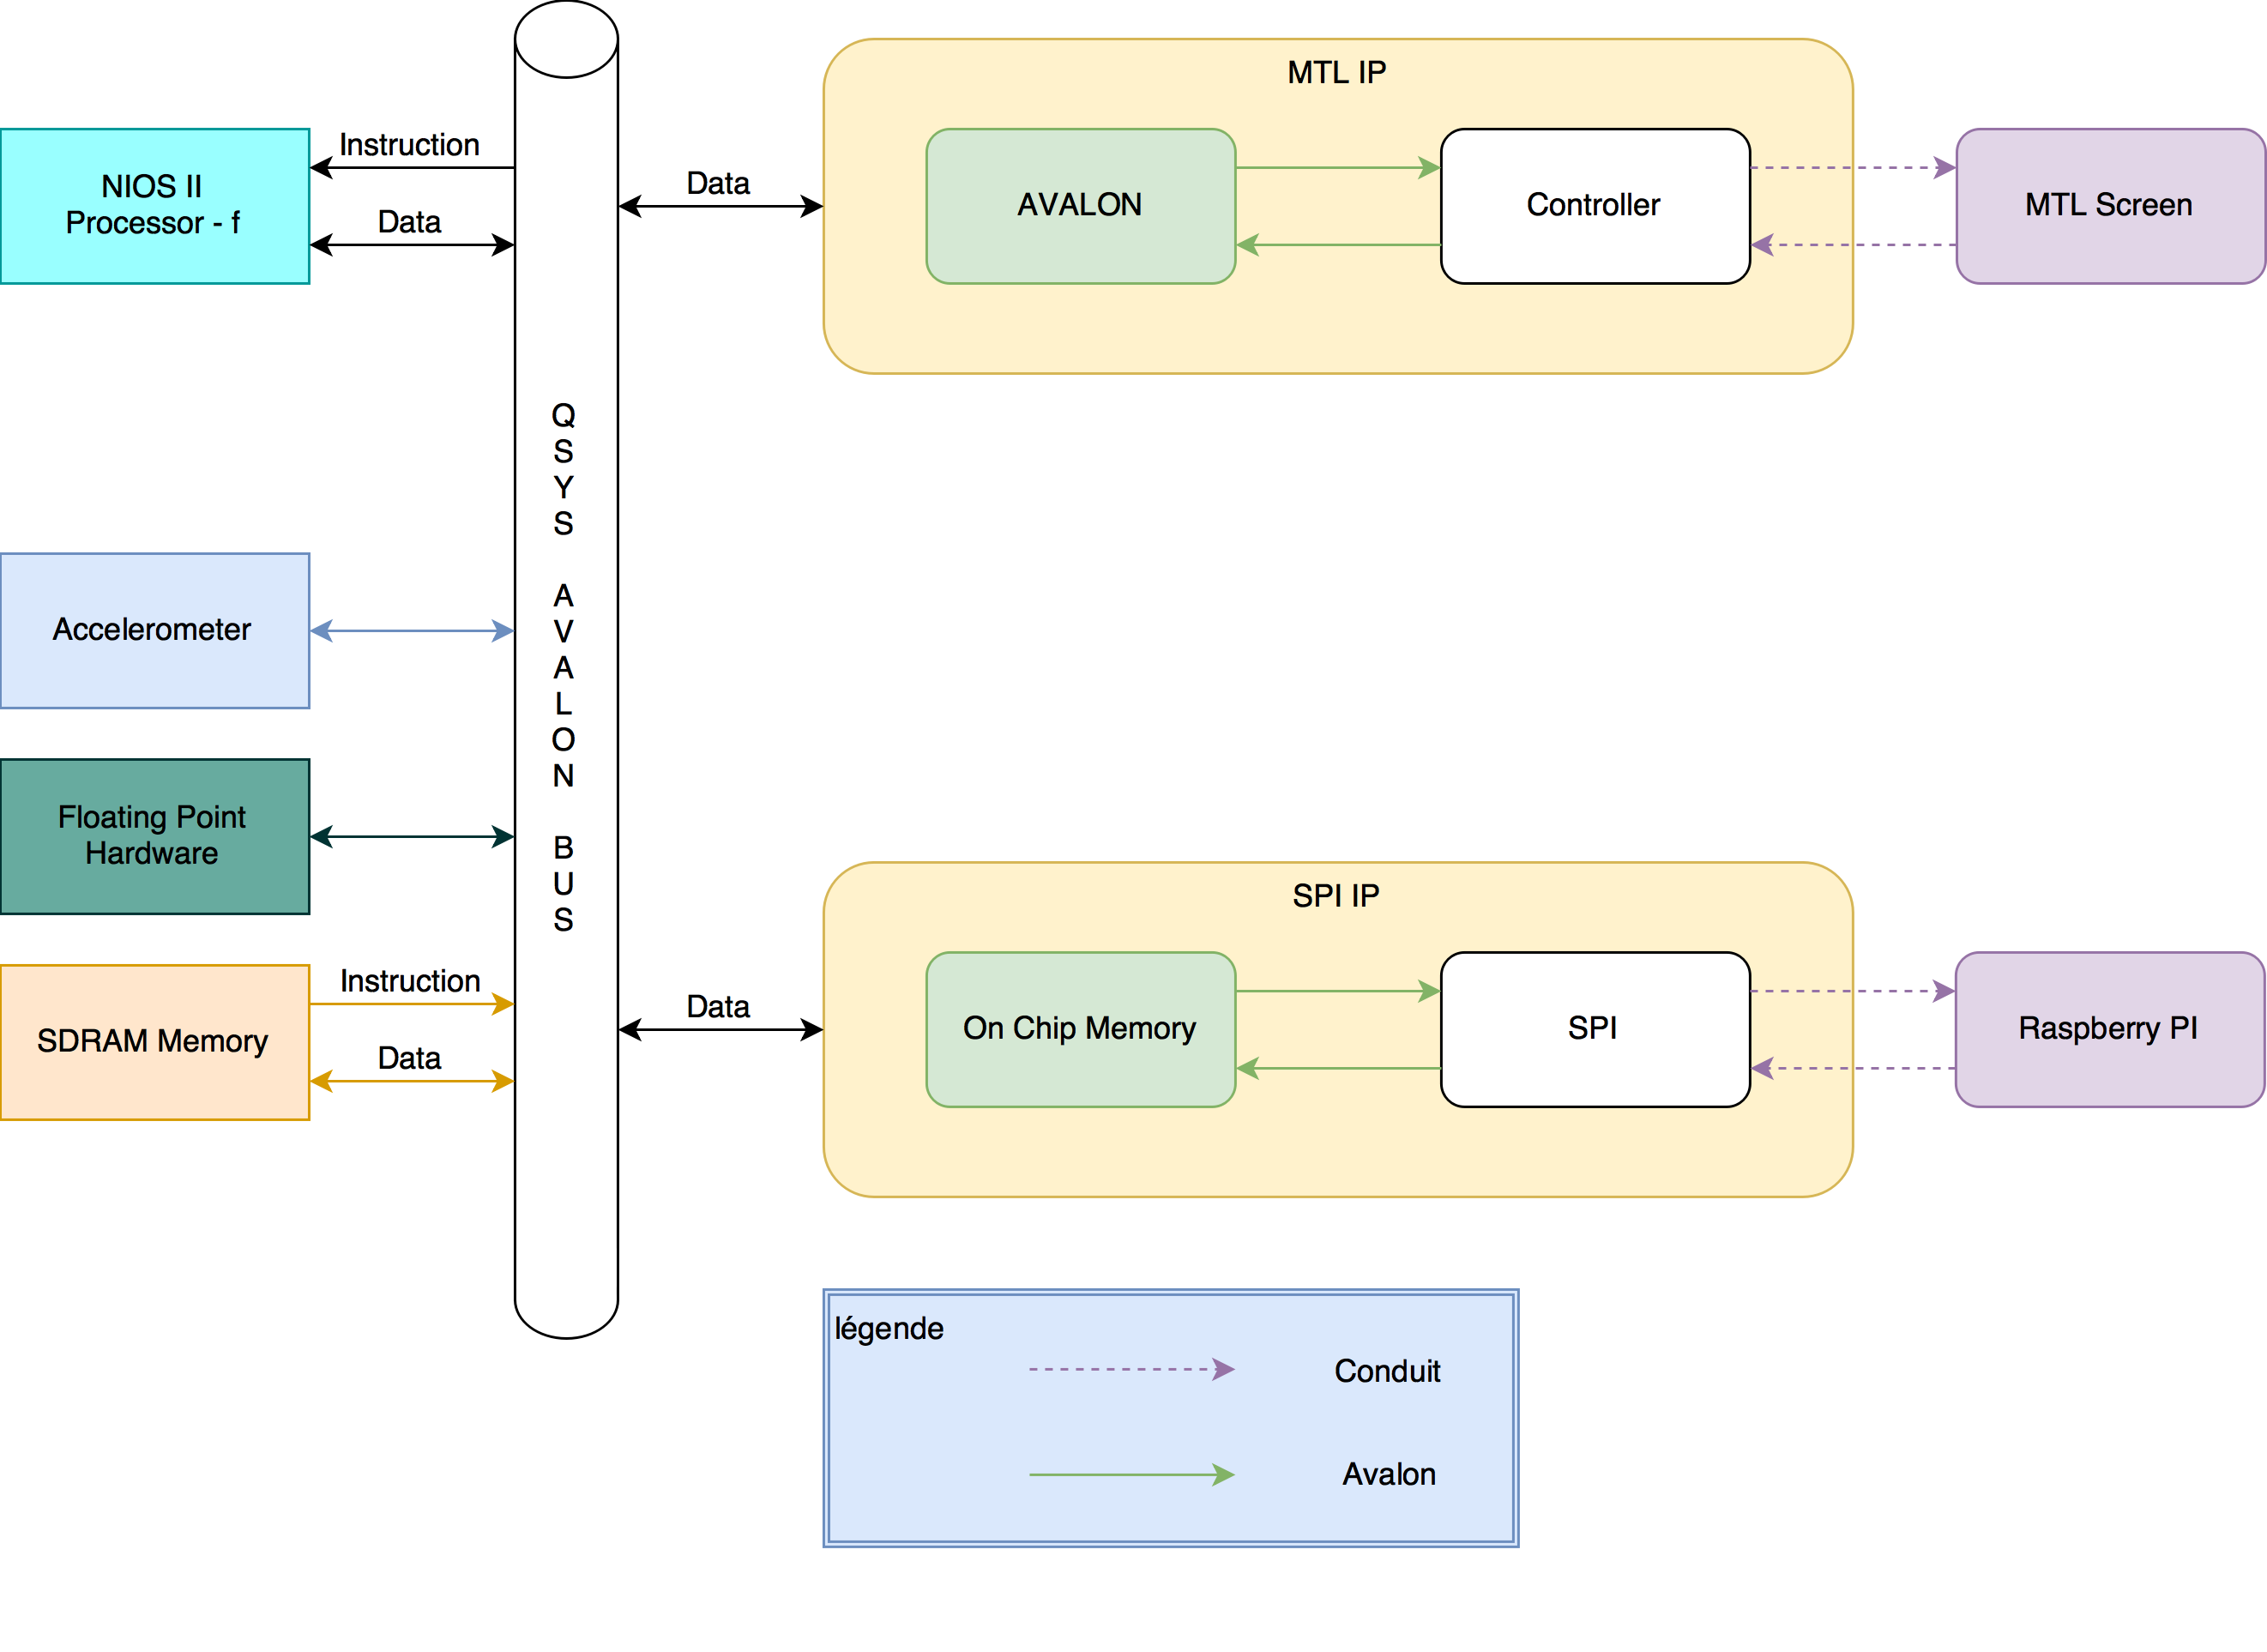
\includegraphics[scale=0.17]{img/Projet_Master.png}
\caption{Shéma générale de la partie hardware}
\label{fig1}

\end{figure}

\end{landscape}

\newpage
\section{Processeur}

Dans cette section, nous allons détailler les choix que nous avons fait dans ce projet au niveau du processeur implémenté en hardware, ainsi que au niveau graphique ainsi que les moyens mis en œuvre pour répondre au objectifs de ce projet. De ce fait, nous nous sommes basé sur le principe même de notre jeu.

\paragraph{Choix du processeur}

De part le nombre important de calculs devant être fait par le processeur (tous les calculs liés au système de collision entre les balles, les directions des tirs,...), nous sommes passés sur un processeur de type f. De plus, nous voulions utilise le module "Floating point hardware", pour que les résultats soient calculés plus rapidement.

\paragraph{Floating point hardware}

Durant le cours de Real-Time, nous avons remarqué que faire les calculs en hardware étaient en moyenne 8 fois plus rapide que si ils étaient fait en software. Lorsque ce module est utilisé, toutes les opérations étant faites en software en temps normal, sont remplacées par des customs instructions implémentées directement en hardware.

% pq type f, utilité du FPH, ...
\section{Gestion de l'écran}
% LE MTL IP n'est pas une custom instruction c'est un IP core
En ce qui concerne l'écran, nous avons utilisé un custom IP core appelée "MTL IP" sur le schéma \ref{fig1}. Celui-ci, contient les modules de contrôles et de gestion des gestes liées à la tablette tactile. Nous avons implémente toute la partie graphique du jeu en hardware.

\paragraph{Background}
Comme on peut le voir su la photo \ref{fig2}, le background ressemble bien à une  table de billard. Celui-ci a été implémenté par une succession de couche successive, les unes sur les autres. Les trous sont générées sur base de l'équation d'un cercle. Idem pour les balles qui vont servir au jeu, elles sont définies par la même equation que les trous, avec un diamètre diffèrent et différentes couleurs définies par leurs valeurs RGB.

\begin{figure}[!ht]
\centering
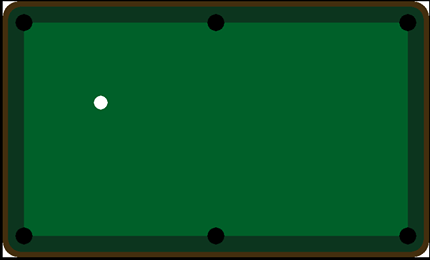
\includegraphics[scale=0.75]{img/background.png}
\caption{Background du jeu}
\label{fig2}
\end{figure}

% ROM, Background, ....

\paragraph{ROM}

Pour faire une sorte de menu de début de jeu, nous avons utilisé des ROMS. Ceci grâce au module Qsys, en lui donnant le bon fichier hexadécimale. La ROM1 est représenté sur la figure \ref{fig3}, et est l'écran d’accueil du jeu. La ROM2, de la figure \ref{fig4}, est l'écran permettant de déterminer lequel des 2 joueurs jouera en premier (celui qui touche en premier l'écran), et  permet également d'être sur que les 2 systèmes (joueur 1 et 2) commencent la partie de manière synchrone.

\begin{figure}[!ht]
   \begin{minipage}[c]{.46\linewidth}
      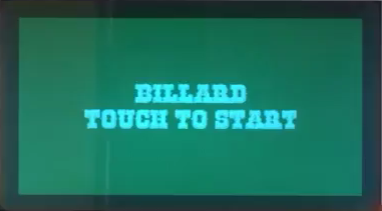
\includegraphics[scale=0.65]{img/start.png}
      \caption{ROM1 - Ecran de demarrage}
      \label{fig3}
   \end{minipage} \hfill
   \begin{minipage}[c]{.46\linewidth}
      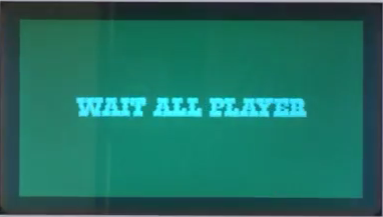
\includegraphics[scale=0.65]{img/Wait_all_player.png}
      \caption{ROM2 - Ecran d'attente des joueurs
      \label{fig4}}
   \end{minipage}
\end{figure}

\paragraph{Gestions des gestes}

Un des objectifs de ce projet était bien sur de développer un nouveau gestes propre à notre jeu. Celui-ci a été implémente pour déterminer la direction dans laquelle la boule blanche va être envoyé ainsi que sa vitesse. 

\begin{figure}[!ht]
\centering
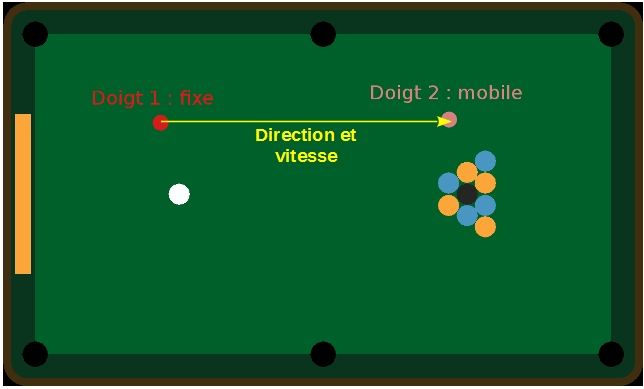
\includegraphics[scale=0.6]{img/gesture.png}
\caption{Illustration du nouveau geste implementé}
\label{fig5}
\end{figure}

Le geste est simple. Il y a 3 détections sur l'écran. Le premier doigt donne l'origine du vecteur de mouvement. Ensuite, le deuxième doigt touche l'écran à l'endroit où on veut que la boule  aille. Enfin, il suffit de retirer le dernier doigt en contact avec la tablette pour valider le coup. Ce mécanisme est illustré sur la figure \ref{fig5}. Pour résume, la balle partira dans la direction donne par le vecteur formé par les deux doigts. Et sa vitesse sera déterminée pour l'écart entre les 2 doigts.


\paragraph{Barre de joueur actif}

Afin de rendre le jeu plus agréable à jouer, nous avons ajouté un barrette sur le côté gauche de L’écran (comme encadré en rouge sur la figure \ref{fig6}) pour que les joueurs ait plus facile à savoir lorsque c'est à leur tour de jouer. En fonction du joueur actif, la barrette apparaîtra bleu pour le joueur 1 et orange pour le joueur 2, ou vice-versa.


\begin{figure}[!ht]
\centering
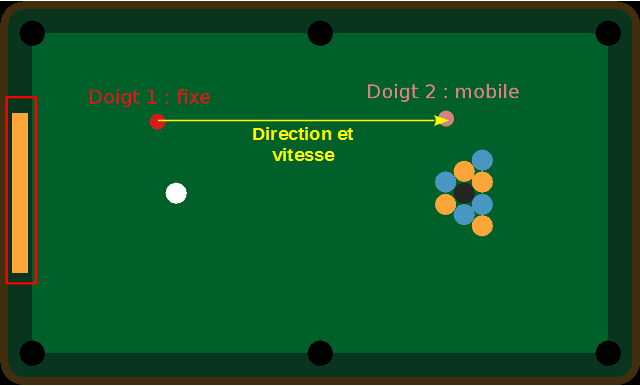
\includegraphics[scale=0.6]{img/barre.png}
\caption{Barre montrant le joueur actif}
\label{fig6}
\end{figure}

\paragraph{Utilisation de l'accéléromètre}

Comme dans tous jeux de billard qui se respecte, l'effet donné a la boule blanche est important. C'est pourquoi nous utilisons l'accéléromètre du FPGA. Comme représente a la figure \ref{fig7}, une fois la direction et la vitesse de la balle décidé, il faut choisir l'effet qu'on veut donner à la balle. Taper à gauche, la fera partir avec un effet à gauche. Il en va de même pour la droite. On peut déplacer le petit point noir en bougeant le FPGA. Ainsi on peut taper n'importe ou sur la boule.

\begin{figure}[!ht]
\centering

\includegraphics[scale=0.6]{img/accel.png}
\caption{Illustration du moyen utilisé pour mettre de l'effet dans la boule blanche}
\label{fig7}
\end{figure}
\newpage
\section{Communication avec le Raspbery-Pi}

Dans ce projet, nous avons utilisé le FPGA que nous avons programmé, mais aussi le Raspberry-PI, et les 2 communiquent via SPI (celui-ci est représente par le custom IP core "SPI IP" sur le schéma \ref{fig1}). Le SPI est très important pour aller lire ou écrire dans les différents registres où se trouve les directions, les vitesses, les valeurs de l'accéléromètre,...Tous ces registres sont bien sur localisés à des adresses préalablement attribuées en hardware, et qu'on atteint grâce au pointeurs présents en software. On peut distinguer 2 cas

\paragraph{Envoi des données}

Dans ce cas-ci, nous devons écrire aux bonnes adresses les valeurs en software. Et ensuite, via SPI, on va lire ces valeurs afin de les transmettre.

\paragraph{Réception des données}

Le principe est à peu près le même que lorsqu'on envoi. En effet, lors de la réception de données, on écrit aux adresses les valeurs reçues, et on les lit grâce au pointeurs en software afin de les utiliser dans les différentes tâches.


\chapter{Partie Software - Real-Time}

\section{Description des 4 tâches}

\begin{figure}[!ht]
\centering
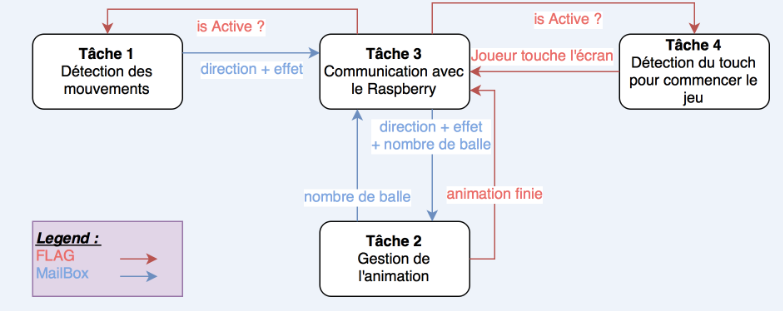
\includegraphics[scale=0.7]{img/task.png}
\caption{Illustration des différentes tâches}
\label{fig8}
\end{figure}

Dans ce projet, nous avons eu recours a plusieurs reprises au notion vues dans le cours de Real-Time. Ce qui explique une utilisation relativement poussée des \textbf{tâches}. En effet, chacune d'elle à un rôle bien particulier.

\paragraph{Tâche 1}

La tâche 1 a pour mission de détecter le geste (décrit dans la section précédente) fait par le joueur sur la tablette. Celle-ci détermine la direction et la vitesse qui seront donnés à la boule blanche lors du tir. Ces deux informations sont transmises à la tâche 3 via Mailboxes. De plus, celle-ci est contrôle par un flag (isActive) pour que celle-ci soit active (quand le joueur joue) ou inactive (quand le joueur ne joue pas).

\paragraph{Tâche 2}

Une des tâches qui fait le plus de calcul. En effet, c'est dans celle-ci que les détection de collisions sont faites, ainsi que les calculs des vitesses et directions des boules lorsqu'il y a collision,... Les valeurs utiles pour ces opérations sont transmises par la tâche 3 via Mailboxes. 

\paragraph{Tâche 3}

C'est cette tâche qui est en communication avec le Raspberry-PI. En effet, celle-ci reçoit les informations (directions, vitesses,...) et les écrits aux adresses qui vont être lues via SPI avant d'être transmises via WIFI. C'est aussi elle qui décide lorsque les tâches 1 et 4 doivent être actives ou pas. C'est aussi elle qui transmet toutes les valeurs  utiles à la tâche 2 aussi bien en envoi que en réception. 

\paragraph{Tâche 4}














\section{Physique}
	\subsection{Collision}
	\subsection{Tir}

\chapter{Communication}
 % DE0-Nano -> R-Pi; R-Pi -> Server
\chapter{Conclusion}
\end{document}